%\documentclass{beamer}
%\usetheme{Pittsburgh}
\documentclass{scrartcl}

\usepackage[utf8]{inputenc}
\usepackage{default}
\usepackage[procnames]{listings}
\usepackage{graphicx}
%\usepackage[toc,page]{appendix}
\usepackage{caption}
\usepackage{hyperref}
\usepackage{color}
%\usepackage{csvsimple}
\usepackage{float}
%\usepackage[T1]{fontenc}



%Bibliogrpahy?
%\usepackage{bibentry}
%\nobibliography*
%\bibentry{ }


%Python
\definecolor{keywords}{RGB}{255,0,90}
\definecolor{comments}{RGB}{0,0,113}
\definecolor{red}{RGB}{160,0,0}
\definecolor{green}{RGB}{0,150,0}
\lstset{language=Python,
    basicstyle=\ttfamily\scriptsize,
    keywordstyle=\color{keywords},
    commentstyle=\color{comments},
    stringstyle=\color{red},
    identifierstyle=\color{green},
    breaklines = true,
    columns=fullflexible,
    %Numbering and tabs
    %numbers=left,
    %numberstyle=\tiny\color{gray},
    %stepnumber=2,
    %numbersep=1em,
    tabsize=4,
    showspaces=false,
    showstringspaces=false}

\begin{document}

\title{Learning and Adaptivity}
\subtitle{Report No. 2}
\author{
  \href{daiem.ali@smail.inf.h-brs.de}{Ali, Daiem}: \href{https://github.com/daiemna}{github.com/daiemna}\\
  \href{christophe.quignon@smail.inf.h-brs.de}{Quignon, Christophe}:\href{https://github.com/ChrisQuignon}{github.com/ChrisQuignon}
  %Familyname, Name
}
\date{\today}


\maketitle

%TODO: add abstract and conclusion
%labels (or zero)
%references (or zero)
%remove scaffolding code


\begin{abstract}
%TODO :review this!
\textbf{Abstract:} This week we analysed our heat-pump data which was collected using sensors over six months. We evaluated the relationship between different features using correlation. Also, we visualized the features in a single graph to verify the hypothesis of their relationship. In the method section there is a use case for heat-pump data usage and a short literature review about the use of decision tree forest in time-series data analysis.
\end{abstract}


\section{Project introduction}
%Include an introduction section to your project

Heat pumps are a sustainable way to transfer thermal energy into out away from builds to keep a comfortable temperature. But to operate a heating pump is not a trivial task, different building distribute the heat differently and weather with its chaotic nature has a major influence on the temperature flow. In addition, they suffer from a suboptimal efficiency because they often have a bad time delay from sensing to acting. This could be counteracted by predicting future temperatures to overact sensors. efficiency could be increased by predicting energy consumption and delay that to times where energy is cheap. 
Thus we want to predict the behaviour or an energy pump with respect to the weather.


\section{Features}
% Include information on which features are available from your data, and include visualizations
For time-series prediction, the features naturally come with the data. On our case, we have the power and energy (Figure \ref{fig:powerenergy}), the volumetric flow rate (Figure\ref{fig:volumetric_flow}), three temperatures (Figure \ref{fig:temperatures} and the relative air humidity and precipitation as in Figure \ref{fig:humidity}.\\
Of those, the outside temperature, the air humidity and the precipitation is the systems input, the input and output temperature and the volumetric flow rate can be thought of as the state of the machine and the energy and power is the output, which we want to predict.\\
This separation however is not as static as presented, and the input temperature can also be thought of as an input, while the volumetric flow rate could also be output.\\
It is also notable that some the values are more closely related then others. The outside temperature naturally tends to drop while it is raining, and the input and output temperature are often substracted to get an easy overview of the system temperature modulation. And the power and energy often highly correlate. Figure\ref{fig:correlate} shows the correlation of the features from which we might decide to merge or drop certain features.\footnotetext{Energie = energy, Niederschlag = precipitation, Rücklauftemperatur = output temperature, Aussentemperatur = outside temperature, Relative Feuchte = relative air humidity, Leistung = power, Volumenstrom = volumetric flow rate, Vorlauftemperatur = input temperature}

\begin{figure}[H]
  \centering
  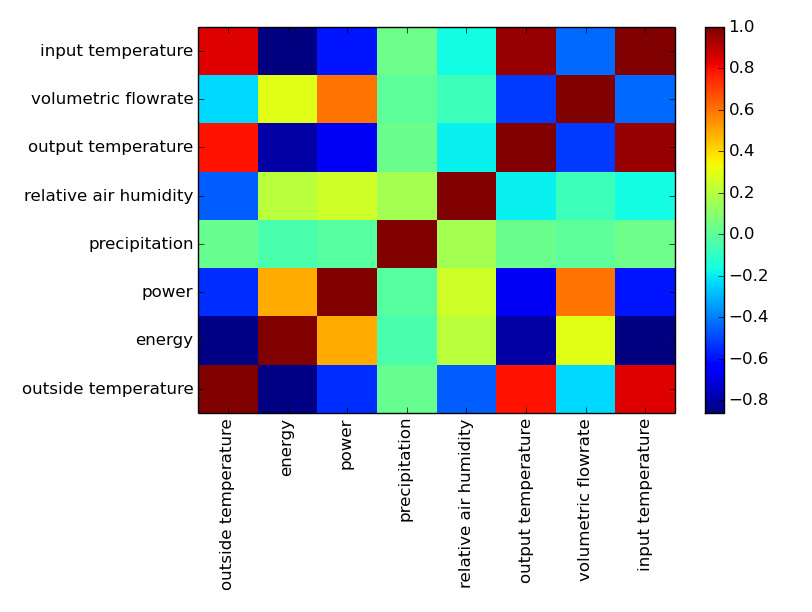
\includegraphics[width=0.5\linewidth]{img/corrmatrix.png}
  \caption[This is needed]{Correlations of the features.\footnotemark}
  \label{fig:correlate}
\end{figure}



\begin{figure}[H]
  \centering
  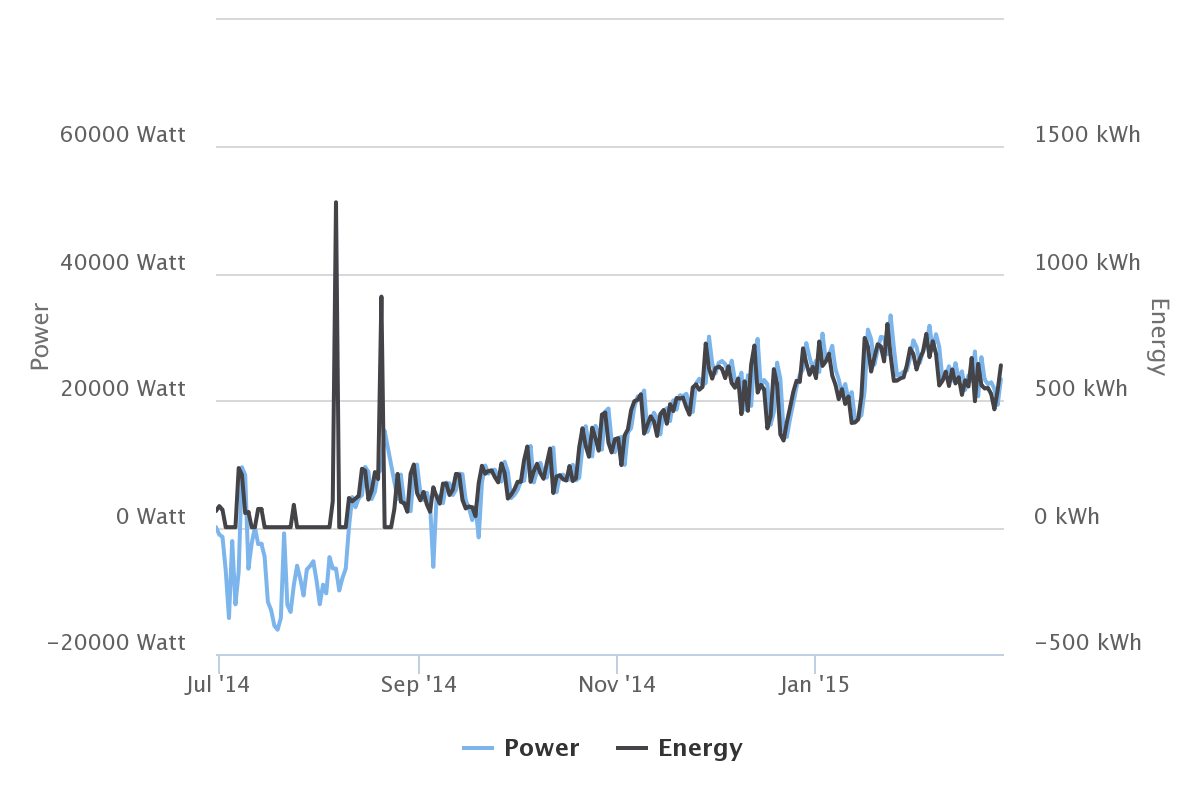
\includegraphics[width=0.8\linewidth]{img/powerenergy.png}
  \caption{Data visualisation of the power and energy}
  \label{fig:powerenergy}
\end{figure}

\begin{figure}[H]
  \centering
  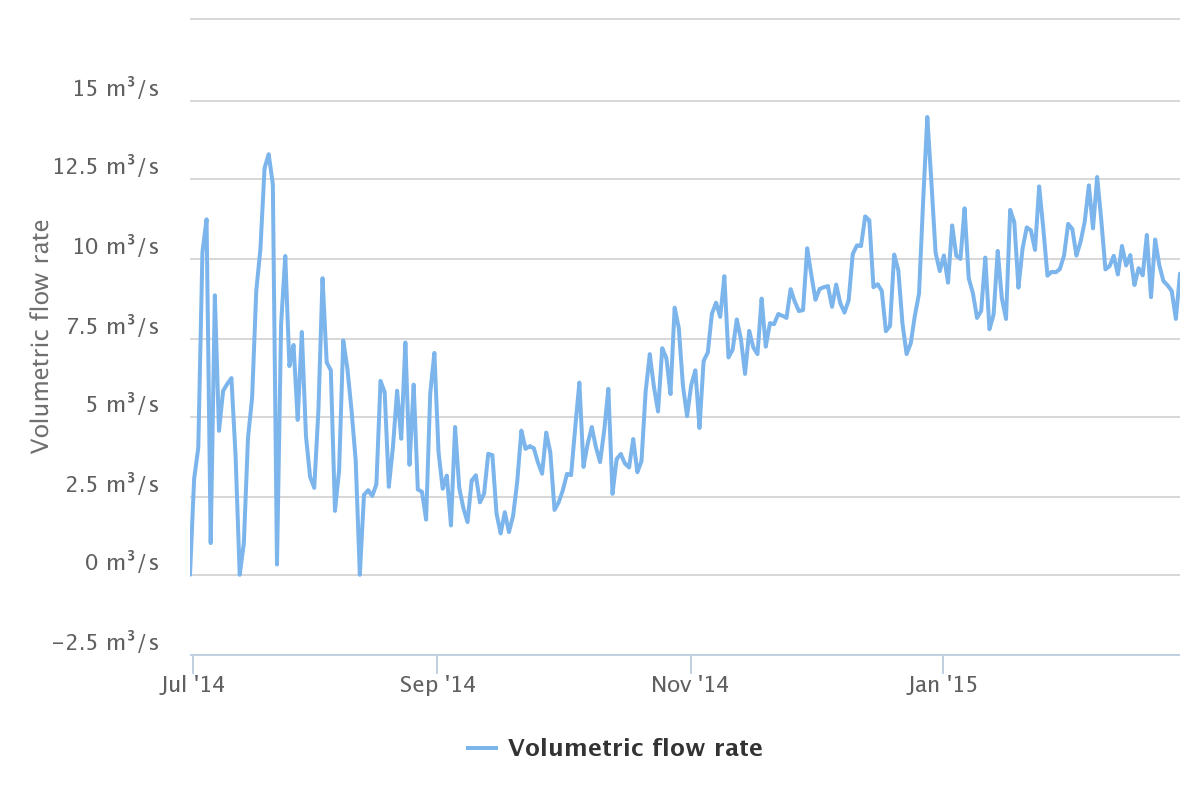
\includegraphics[width=0.8\linewidth]{img/Volumetric_flow.png}
  \caption{Data visualisation of the volumetric flow rate.}
  \label{fig:volumetric_flow}
\end{figure}

\begin{figure}[H]
  \centering
  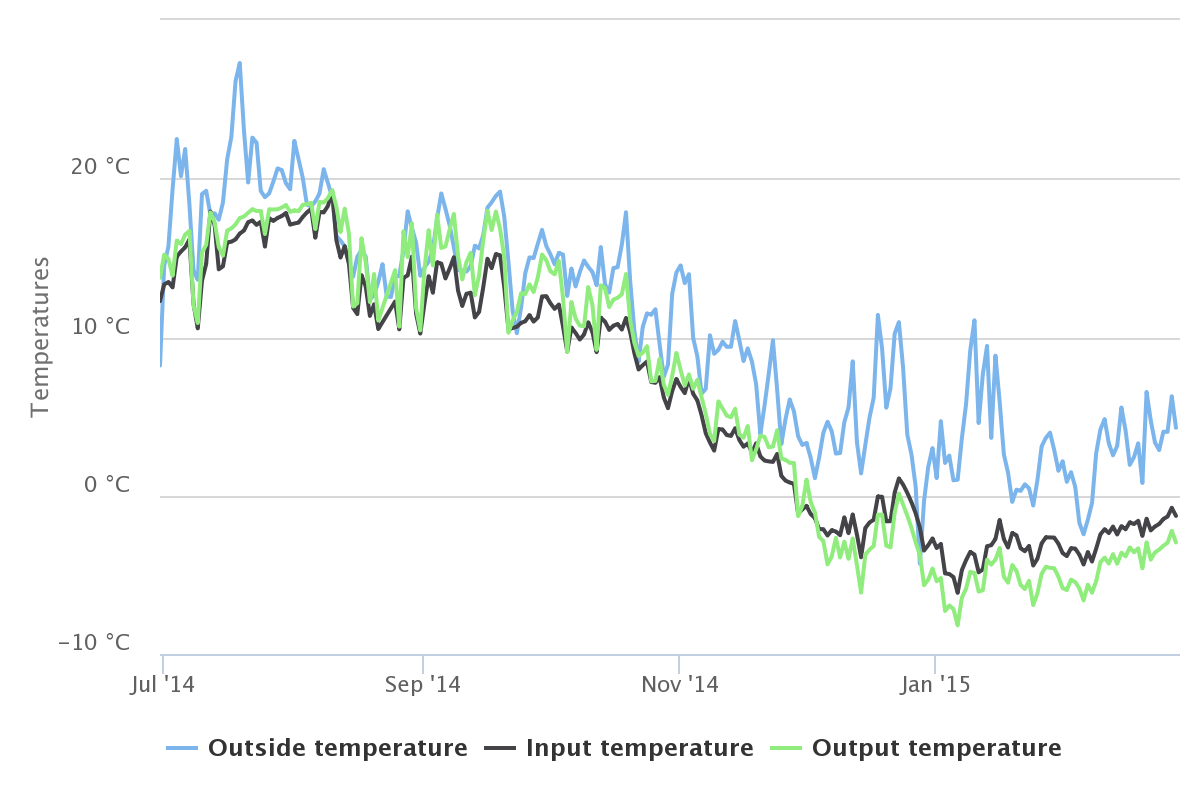
\includegraphics[width=0.8\linewidth]{img/Temperatures.png}
  \caption{Data visualisation of the temperature outside, the temperature input and the temperature output.}
  \label{fig:temperatures}
\end{figure}

\begin{figure}[H]
  \centering
  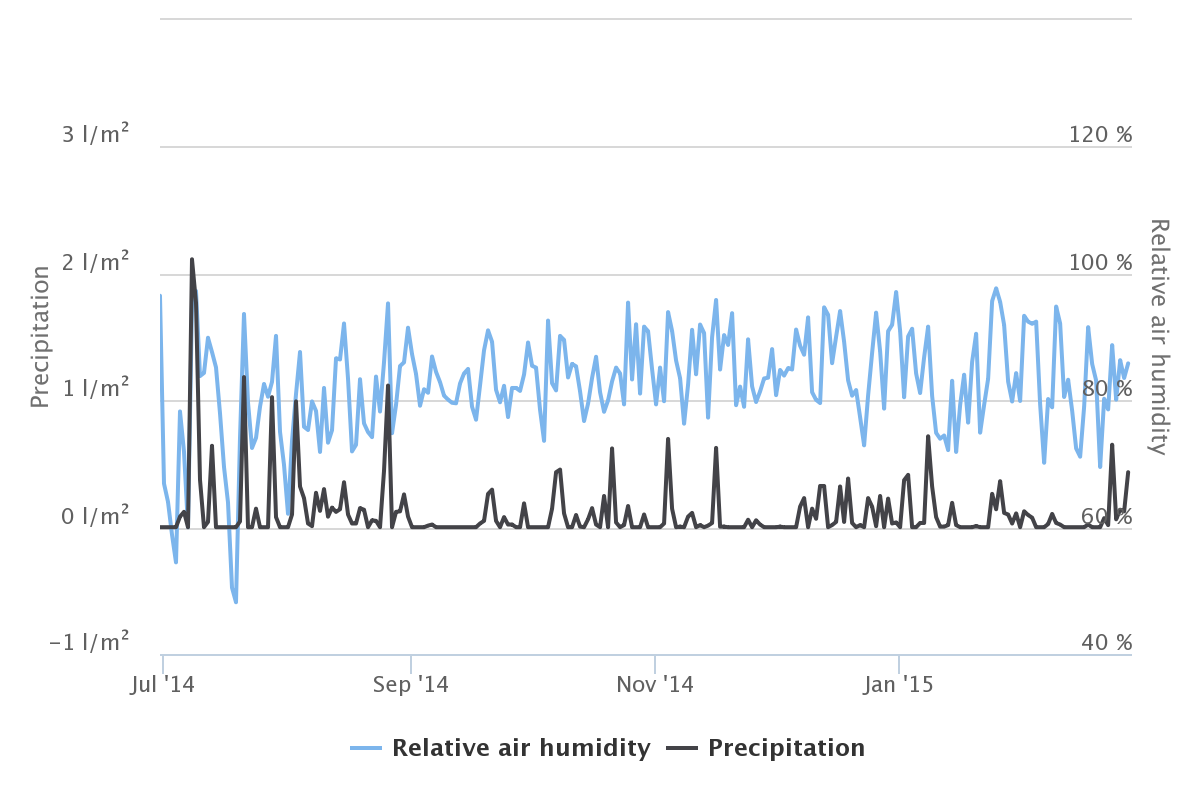
\includegraphics[width=0.8\linewidth]{img/humidity.png}
  \caption{Data visualisation of the relative air humidity and precipitation.}
  \label{fig:humidity}
\end{figure}


\section{Method}
%Include a section on what Machine Learning method you intend to use, and why you believe it will be suitable for your data.
Right now, heat-pumps are often controlled by hand. A set of predefined rules may set off an alarm to the operator who then can react. These rule are often thresholds, that is either directly read from a sensor or collected from different sensors. To ensure a smooth transition and a correct prediction behaviour, we want to model those rules as accurate as possible. As a first transition step, the rules used for prediction can be set into the existing system for testing. The operator and the performance of the system with those rules can give valuable information for a good prediction performance.\\
Decision trees closely resemble those simple rules, and have the advantage that the prediction output is human readable and can be checked by the operator. To improve the precision of the decision tree, multiple randomly initiated decision trees are set up in a random forest. Those random forests average the outcome of all decision trees. Classically, decision trees are used for classification, but they can be adapted for forecasting as shown in \cite{pant1990innocents}. For stock market prediction, their performance is comparable with Support Vector Machines and can be superior to Neural Networks as shown in \cite{kumar2006forecasting}. However, they need fine-tuning and also default settings do not guarantee good prediction as shown in \cite{segal2004machine}

\section{Conclusion} 
%TODO
%http://blog.kaggle.com/2012/05/01/chucking-everything-into-a-random-forest-ben-hamner-on-winning-the-air-quality-prediction-hackathon/


%BIBLIOGRPAHY?
\bibliographystyle{plain}%amsalpha
\bibliography{bib.bib}
%\bibentry{}

%\begin{appendix}
%\section{}

%\end{appendix}


%COPY AND PASTE FROM HERE

%\begin{enumerate}
% \item
%\end{enumerate}

%\href{link}{text}

%\begin[Language=Python]{lstlisting}
%#PYTHON CODE HERE
%\end{lstlisting}

%\lstinputlisting[language=Python]{	}

%\csvautotabular[separator=semicolon]{data.csv}

%\subsubsection{left}
%\begin{figure}[H]
%  \centering
%  \includegraphics[width=0.5\linewidth]{../img/	}
%  %\caption{}
%  %\label{fig:}
%\end{figure}
%PUT UNITS ON THE FIGURES

\end{document}
